\chapter{Аналитическая часть}

В этой части рассматриваются анализ предметной области, известных решений и моделей баз данных, формализации задачи и ролей.

\section{Анализ предметной области}

Организация мероприятий -- это многогранный и трудоемкий процесс, который требует внимания к деталям и учета множества факторов. От выбора подходящей локации до составления списка гостей, от планирования бюджета до подготовки меню -- каждый этап организации требует тщательной проработки. В ходе подготовки организаторы сталкиваются с рядом типичных вопросов, таких как: «Что необходимо приобрести для мероприятия?», «Какое количество гостей ожидается?» и «Какова стоимость участия?». Эти вопросы, хотя и кажутся простыми, но требуют значительных временных и организационных затрат, особенно если мероприятие масштабное или включает множество участников~\cite{lit1}.

Для упрощения этого процесса были разработаны специализированные инструменты -- планировщики мероприятий. Эти приложения предназначены для того, чтобы объединить все этапы организации мероприятия в единую систему, сделать процесс планирования более структурированным и прозрачным. Планировщик мероприятий позволяет организаторам:
\begin{enumerate}
	\item систематизировать задачи -- разбить процесс организации на этапы и подзадачи;
	\item координировать участников -- вести список гостей, учитывать их предпочтения и информировать о деталях мероприятия;
	\item управлять бюджетом -- учитывать расходы и планировать финансы, чтобы избежать непредвиденных затрат;
	\item контролировать сроки -- устанавливать дедлайны для каждой задачи и отслеживать их выполнение.
\end{enumerate}


\section{Анализ известных решений}

Организация мероприятий всегда была важной и востребованной сферой, потому для упрощения этого процесса были разработаны специализированные информационные системы, которые автоматизируют множество задач. Наиболее популярными являются:
\begin{enumerate}
	\item Eventbrite -- платформа для организации мероприятий, которая позволяет создавать страницы событий, продавать билеты онлайн, собирать данные о посетителях и управлять регистрациями~\cite{lit2};
	\item Cvent -- профессиональная платформа для организации мероприятий, которая предлагает комплексные решения для планирования, управления гостями, бюджетирования и аналитики~\cite{lit3};
	\item Trello -- инструмент для управления проектами и задачами, который можно адаптировать для планирования мероприятий~\cite{lit4}.
\end{enumerate}

Критерии сравнения известных решений и результаты их сравнительного анализа представлены в таблицах~\ref{tbl:criteria} и~\ref{tbl:results} соответственно.

\begin{table}[h]
	\centering
	\caption{Критерии сравнения известных решений}
	\begin{tabularx}{\textwidth}{|X|X|}
		\hline
		\textbf{Критерий} & \textbf{Описание} \\
		\hline
		Аккаунт & Возможность иметь аккаунт \\
		\hline
		Бесплатный доступ & Бесплатный доступ ко всем возможностям приложения \\
		\hline
		Привилегии участников & Возможность выдавать участникам роли с привилегиями \\
		\hline
		Рейтинг & Формирование оценки мероприятия по оставленным отзывам \\
		\hline
	\end{tabularx}
	\label{tbl:criteria}
\end{table}

\begin{table}[h]
	\centering
	\caption{Результаты сравнительного анализа известных решений}
	\begin{tabularx}{\textwidth}{|X|X|X|X|}
		\hline
		\textbf{Критерий} & \textbf{Eventbrite} & \textbf{Cvent} & \textbf{Trello} \\
		\hline
		Аккаунт & + & + & + \\
		\hline
		Бесплатный доступ & - & - & + \\
		\hline
		Привилегии участников & - & + & - \\
		\hline
		Рейтинг & + & + & - \\
		\hline
	\end{tabularx}
	\label{tbl:results}
\end{table}

Ни одно из рассматриваемых решений не обеспечивает пользователя всеми необходимыми функциями для организации мероприятий.

\section{Формализация задачи}

Необходимо спроектировать и реализовать базу данных, которая будет хранить данные о пользователях, мероприятиях и отзывах. Также требуется разработать приложение с функционалом для просмотра, добавления, редактирования и удаления информации.

\section{Формализация данных}

Исходя из анализа предметной области, можно выделить следующие ключевые группы данных:
\begin{itemize}[label=--]
	\item локация;
	\item мероприятие;
	\item день мероприятия;
	\item участник мероприятия;
	\item меню мероприятия;
	\item предмет меню;
	\item отзыв;
	\item пользователь.
\end{itemize}

Группы данных и сведения о них представлены в таблице~\ref{tbl:data-groups}

\begin{table}[h]
	\centering
	\caption{Группы данных и их сведения}
	\begin{tabularx}{\textwidth}{|X|X|}
		\hline
		\textbf{Группа данных} & \textbf{Сведения} \\
		\hline
		Локация & Название, описание, цена аренды, вместимость \\
		\hline
		Мероприятие & Название, описание, дата, количество участников, количество дней, локация, рейтинг \\
		\hline
		День мероприятия & Название, порядковый номер, описание, цена посещения, меню \\
		\hline
		Отзыв & Комментарий, рейтинг, участник мероприятия \\
		\hline
		Пользователь & Имя, телефон, гендер, роль, права доступа, пароль \\
		\hline
		Участник мероприятия & Имя, тип, факт оплаты \\
		\hline
		Меню мероприятия & Название, стоимость \\
		\hline
		Предмет меню & Название, тип, цена \\
		\hline
	\end{tabularx}
	\label{tbl:data-groups}
\end{table}

\newpage

ER-диаграмма сущностей в нотации Чена представлена на рисунке~\ref{fig:er-diagram}.

\begin{figure}[h]
	\centering
	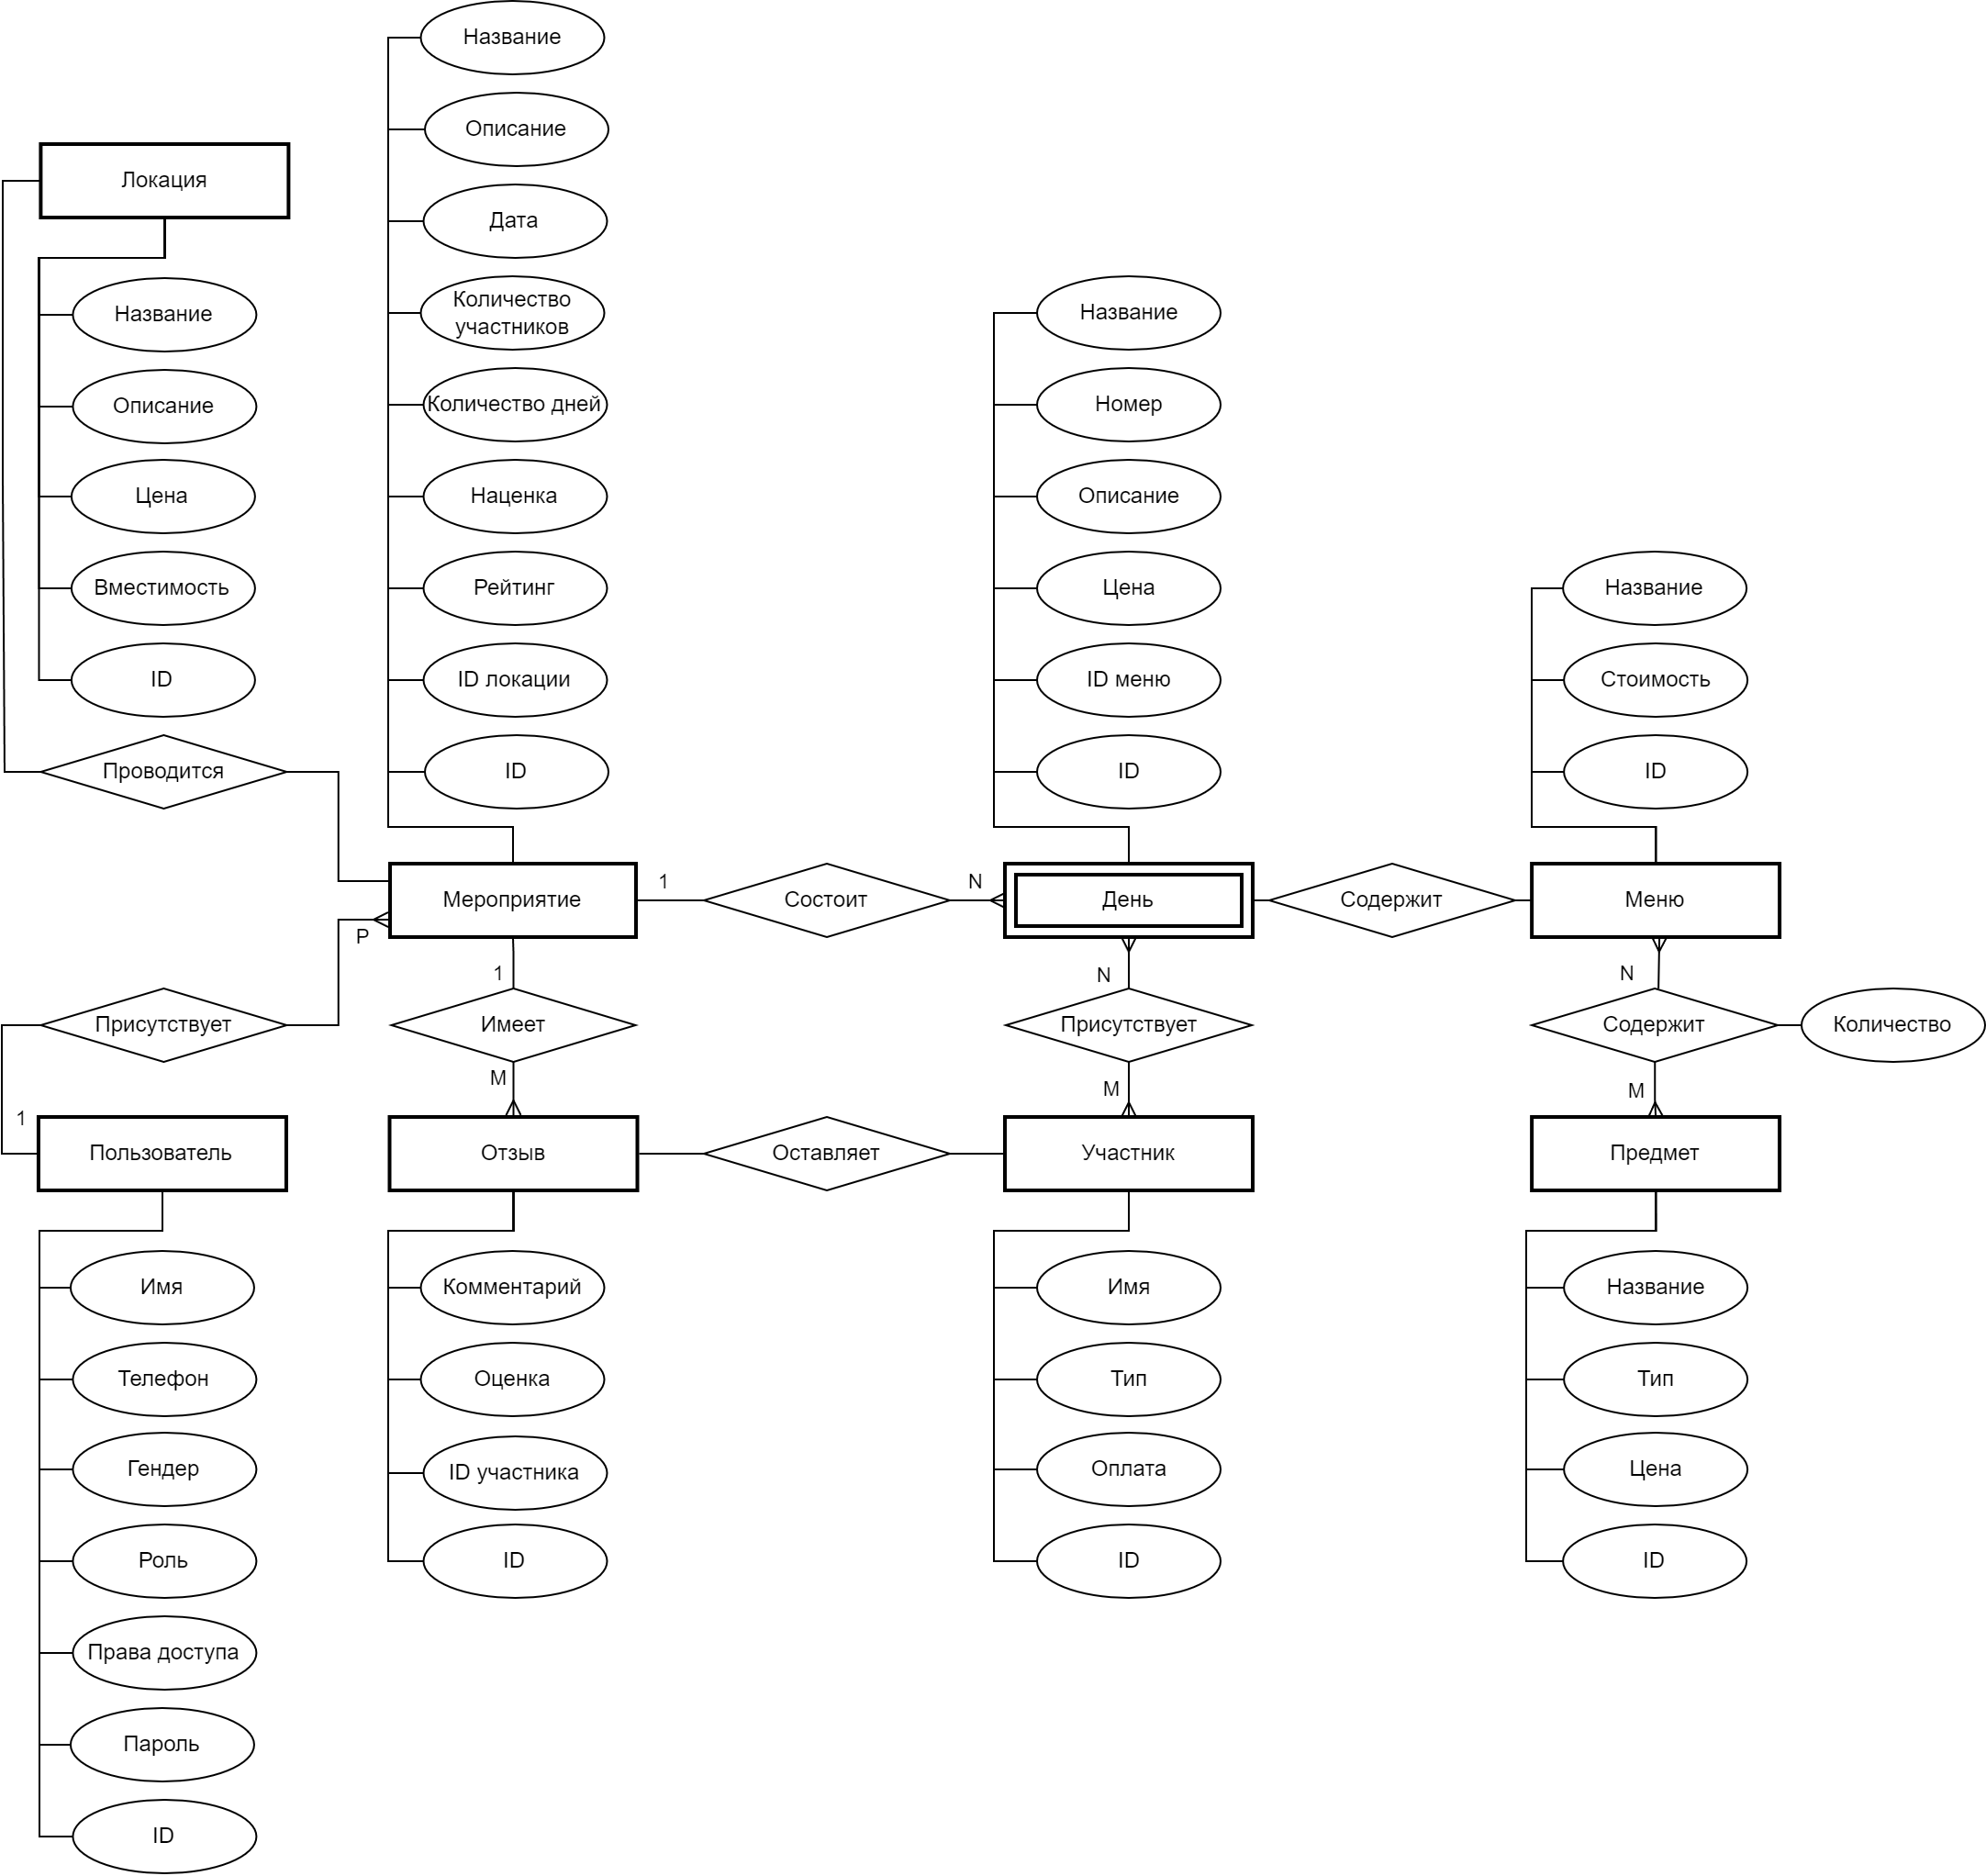
\includegraphics[width=1\textwidth]{images/er-diagram.png}
	\caption{ER-диаграмма сущностей в нотации Чена} 
	\label{fig:er-diagram} 
\end{figure}

\newpage

\section{Формализация ролей и типов}

Множества значений перечисляемых сведений представлены в таблице~\ref{tbl:data-groups-types}.

\begin{table}[h]
	\centering
	\caption{Множества значений перечисляемых сведений}
	\begin{tabularx}{\textwidth}{|p{5cm}|p{2cm}|X|}
		\hline
		\textbf{Группа данных} & \textbf{Сведение} & \textbf{Множество значений} \\
		\hline
		Пользователь & Роль & Гость, зарегистрированный пользователь, администратор \\
		\cline{2-3}
		& Гендер & Мужской, женский \\
		\hline
		Участник мероприятия & Тип & Простой участник, VIP, организатор \\
		\hline
		Предмет меню & Тип & Однодневный, многодневный \\
		\hline
	\end{tabularx}
	\label{tbl:data-groups-types}
\end{table}


Роли пользователей, выделяемые в разрабатываемой системе, представлены в таблице~\ref{tbl:user-roles}.

\begin{table}[h]
	\centering
	\caption{Категории пользователей}
	\begin{tabularx}{\textwidth}{|p{5cm}|X|}
		\hline
		\textbf{Роль} & \textbf{Описание} \\
		\hline
		Гость & Неавторизованный пользователь, который может регистрироваться, входить в систему и просматривать информацию о мероприятиях \\
		\hline
		Зарегистрированный пользователь & Может просматривать данные о мероприятиях, подавать и удалять заявки на участие, а также оставлять и удалять отзывы \\
		\hline
		Администратор & Обладает правами на просмотр, добавление и изменение данных о мероприятиях, пользователях и отзыва. \\
		\hline
	\end{tabularx}
	\label{tbl:user-roles}
\end{table}

Типы участников, выделяемые в рамках мероприятия, представлены в таблице~\ref{tbl:person-types}.

\begin{table}[h]
	\centering
	\caption{Типы участников}
	\begin{tabularx}{\textwidth}{|p{5cm}|X|}
		\hline
		\textbf{Тип} & \textbf{Описание} \\
		\hline
		Простой участник & Не имеет специальных прав или привилегий \\
		\hline
		VIP-персона & Присутствует на мероприятии бесплатно \\
		\hline
		Организатор & Имеет доступ ко всей информации о мероприятии и присутствует на нём бесплатно \\
		\hline
	\end{tabularx}
	\label{tbl:person-types}
\end{table}

\newpage

Типы предметов, выделяемые в рамках меню, представлены в таблице~\ref{tbl:items-types}.

\begin{table}[h]
	\centering
	\caption{Типы предметов}
	\begin{tabularx}{\textwidth}{|p{5cm}|X|}
		\hline
		\textbf{Тип} & \textbf{Описание} \\
		\hline
		Однодневный & Требуется только для одного дня мероприятия \\
		\hline
		Многодневный & Необходим на протяжении всего мероприятия \\
		\hline
	\end{tabularx}
	\label{tbl:items-types}
\end{table}

\section{Анализ моделей баз данных}

База данных -- самодокументированное собрание интегрированных записей. Она служит основой для хранения, обработки и анализа информации, необходимой для функционирования бизнеса, научных исследований или других сфер деятельности. В зависимости от типа задач, базы данных могут быть классифицированы на два основных типа~\cite{lit7, lit8}:
\begin{enumerate}
	\item OLAP (\textit{англ. Online Analytical Processing}) -- технология для многомерного анализа больших объемов данных, используемая для быстрого выполнения сложных запросов;
	\item OLTP (\textit{англ. Online Transaction Processing}) -- система для обработки транзакций в реальном времени, ориентированная на быструю запись и чтение небольших объемов данных.
\end{enumerate}

Система управления базами данных -- приложение, обеспечивающее создание,
хранение, обновление и поиск информации в базах данных~\cite{lit8}.

Основные функции СУБД:
\begin{itemize}[label=--]
	\item управление данными во внешней памяти;
	\item управление буферами оперативной памяти;
	\item управление транзакциями;
	\item журнализация;
	\item поддержка языка или языковых пакетов;
	\item обеспечение целостности и безопасности базы данных.
\end{itemize}

Модель данных -- это структурное представление элементов данных, их отношений и ограничений в системе управления базами данных. Системы управления базами данных  классифицируются по модели данных, которая определяет их архитектуру, структуры данных и методы обработки. 

\newpage

Выделяются три категории моделей~\cite{lit7, lit8}: 
\begin{itemize}[label=--]
	\item дореляционные;
	\item реляционные;
	\item постреляционные.
\end{itemize}

\subsection{Дореляционная модель}

Дореляционные базы данных представляют собой ранние системы управления данными, которые широко использовались до появления реляционной модели. Эти системы, такие как иерархические и сетевые СУБД, были разработаны для организации и хранения данных в сложных структурах, которые отражали специфические взаимосвязи между объектами. Однако, несмотря на свою функциональность, они обладают рядом ограничений, которые делают их менее гибкими и удобными по сравнению с современными реляционными базами данных~\cite{lit7}.

Иерархические базы данных используют дерево, где каждый элемент данных (узел) имеет строгую связь <<родитель-потомок>>. Такая организация эффективна для данных, которые естественным образом поддаются иерархическому представлению, например, файловые системы или организационные структуры компаний. Однако главным недостатком иерархических моделей является их неэффективность: доступ к данным часто требует обхода всей структуры, что усложняет выполнение запросов.

Сетевые базы данных являются развитием иерархических моделей, устраняя некоторые их ограничения. В сетевых моделях данные организовываются в виде графа, где узлы могут иметь множественные связи друг с другом. Это позволяет более гибко представлять сложные взаимосвязи между объектами, что делает их подходящими для задач, где данные имеют множество пересекающихся связей. Однако, несмотря на большую универсальность, сетевые модели остаются сложными в проектировании и использовании.

Хотя дореляционные модели хорошо справляются с управлением памятью, их применение осложняется зависимостью от физической структуры данных, что делает процесс внесения изменений в базу данных более трудоёмким.

\newpage

\begin{figure}[h]
	\centering
	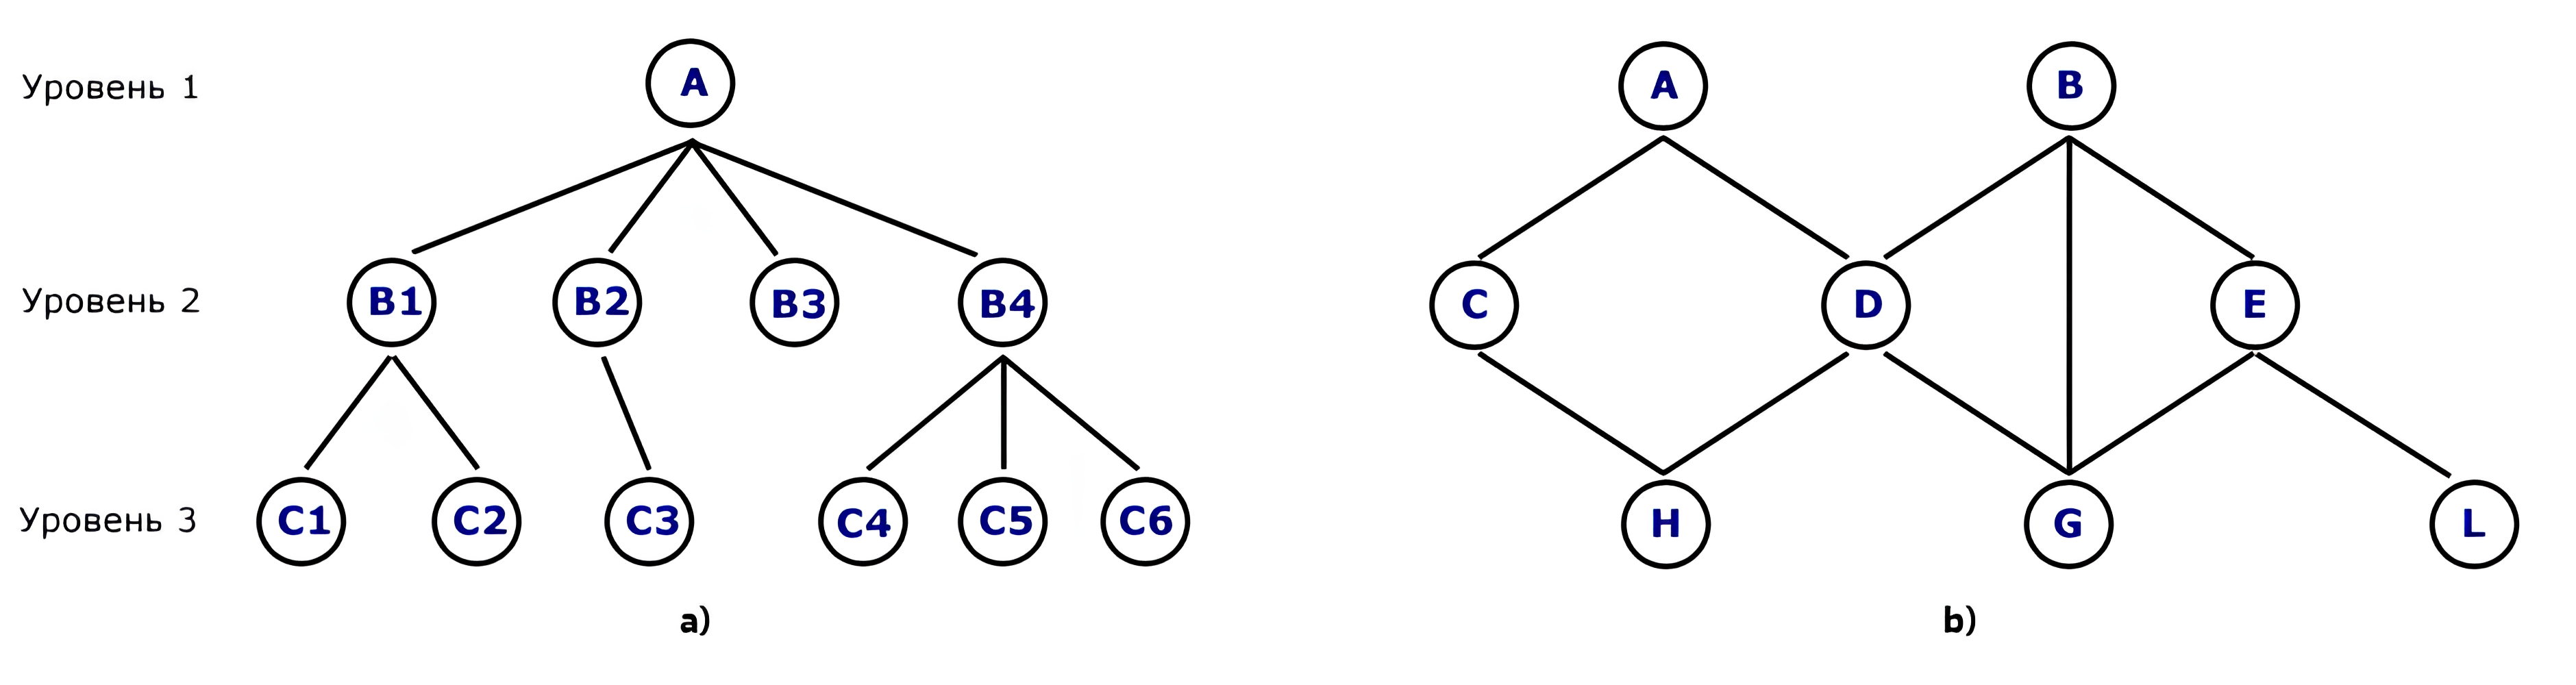
\includegraphics[width=1\textwidth]{images/prerelational-model.png}
	\caption{Структуры дореляционных моделей: иерархическая~(a), сетевая~(b)} 
	\label{fig:hierarchy-model} 
\end{figure}

\subsection{Реляционная модель}

Реляционная модель данных включает в себя три части~\cite{lit8}:
\begin{enumerate}
	\item cтруктурная часть -- данные представляются в виде таблиц, называемых отношениями. Каждая таблица состоит из строк (кортежей) и столбцов (атрибутов). Атрибуты имеют определённые домены -- допустимые значения, которые они могут принимать. Ключи (первичные и внешние) обеспечивают уникальность записей и связь между таблицами. Схемы определяют структуру базы данных, включая таблицы, атрибуты и связи между ними;
	\item целостная часть -- определяет правила, которые гарантируют корректность и согласованность данных:
	\begin{itemize}[label=--]
		\item целостность сущностей: каждый кортеж в таблице должен иметь уникальный идентификатор (первичный ключ), что исключает дублирование записей;
		\item целостность ссылок: внешние ключи в одной таблице должны соответствовать первичным ключам в другой, что обеспечивает согласованность данных между таблицами. Это требование поддерживается нормализацией отношений, которая устраняет избыточность данных.
	\end{itemize}
	\item манипуляционная часть -- включает инструменты для работы с данными, такие как реляционная алгебра и реляционное исчисление. Реляционная алгебра основана на теории множеств и предоставляет набор операций (например, выборка, проекция, объединение, разность) для манипуляции данными. Реляционное исчисление, основанное на логике предикатов, позволяет формулировать запросы на декларативном уровне.
\end{enumerate}

Модель отличается простотой, независимостью данных и удобством реализации, но имеет недостатки, такие как сложность описания иерархических связей.

\subsection{Постреляционная модель}

Классическая реляционная модель предполагает, что данные в полях таблиц должны быть неделимыми, что может ограничивать эффективность некоторых приложений. Постреляционная модель устраняет это ограничение, допуская многозначные поля и вложенные таблицы, что упрощает описание сложных структур. Основное преимущество постреляционной модели -- возможность объединять несколько связанных таблиц в одну, что повышает наглядность и ускоряет обработку данных.

\section{Вывод}

В аналитической части работы были проведены анализы предметной области, известных решений и моделей баз данных, проведены формализации задачи, данных и ролей. Был сделан выбор в пользу реляционной модели базы данных.

\clearpage
